\begin{frame}{XOR --- 직선 한 줄로 나눌 수 있을까?}
  \centering
  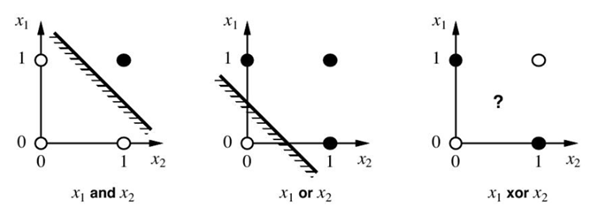
\includegraphics[width=0.85\linewidth]{xor_and_or_xor.png}

  \vskip0.3em
  \small
  \begin{itemize}
    \item \textbf{AND}와 \textbf{OR}: 검은 점과 흰 점을 직선 하나로 가를 수 있다.
    \item \textbf{XOR}(``둘 중 정확히 하나만 1''): 검은 점 두 개가 대각선 모서리에
      놓여, 직선 하나로는 가를 수 없다.
    \item 1969년 민스키·페퍼트가 이 한계를 증명했고, 이것이 첫 번째 음영의 출발점이다.
  \end{itemize}
\end{frame}
